\chapter{Future Work}
\label{chap:6}

\begin{figure}[ht]
\centering
		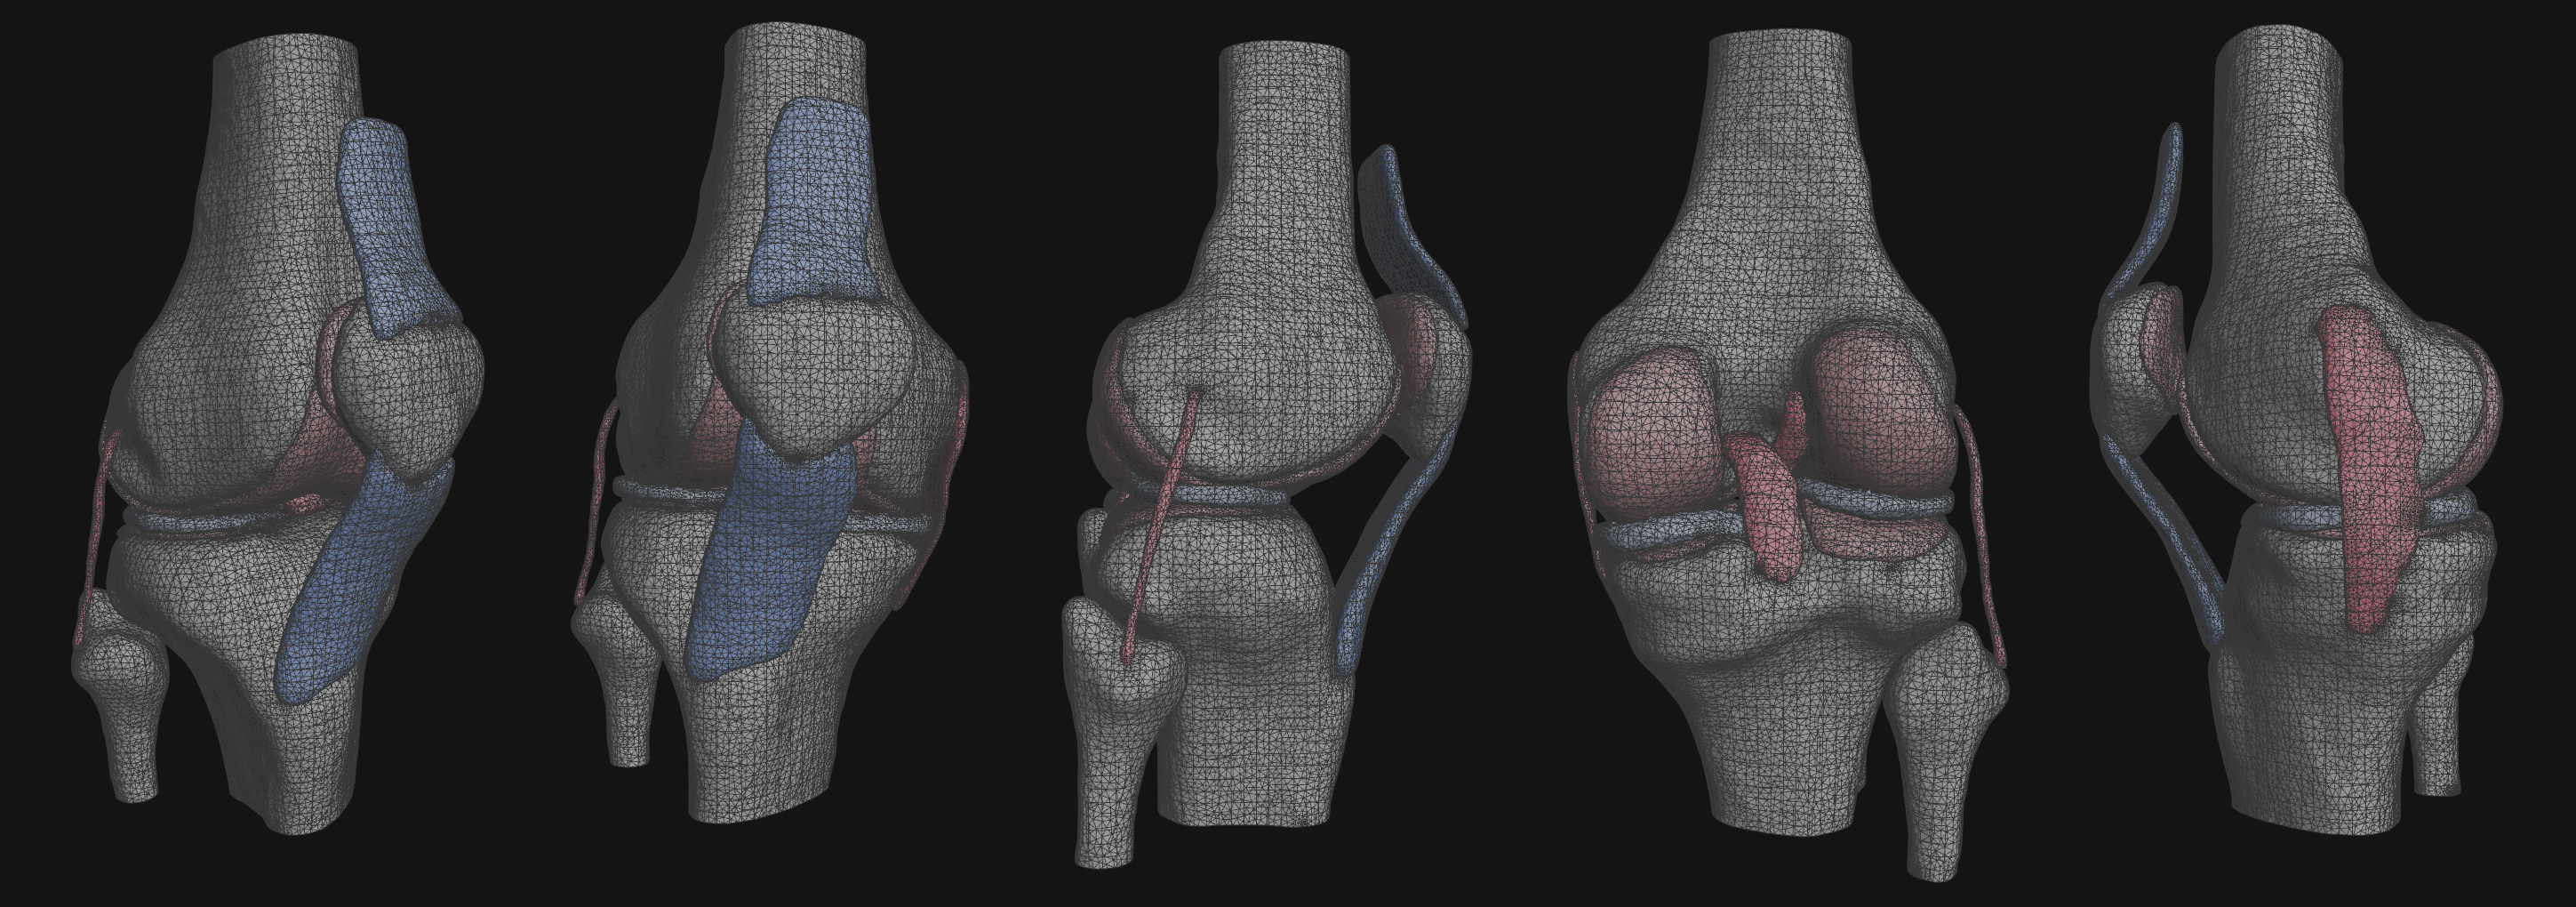
\includegraphics[width=1.0\textwidth]{media/7-polyknee/fullmesh.png}
%
\caption{Polyhedral mesh of human knee from input surfaces generated from OpenKnee image masks}
\label{fig:polyknee}
\end{figure}

\begin{figure}[ht]
\centering
		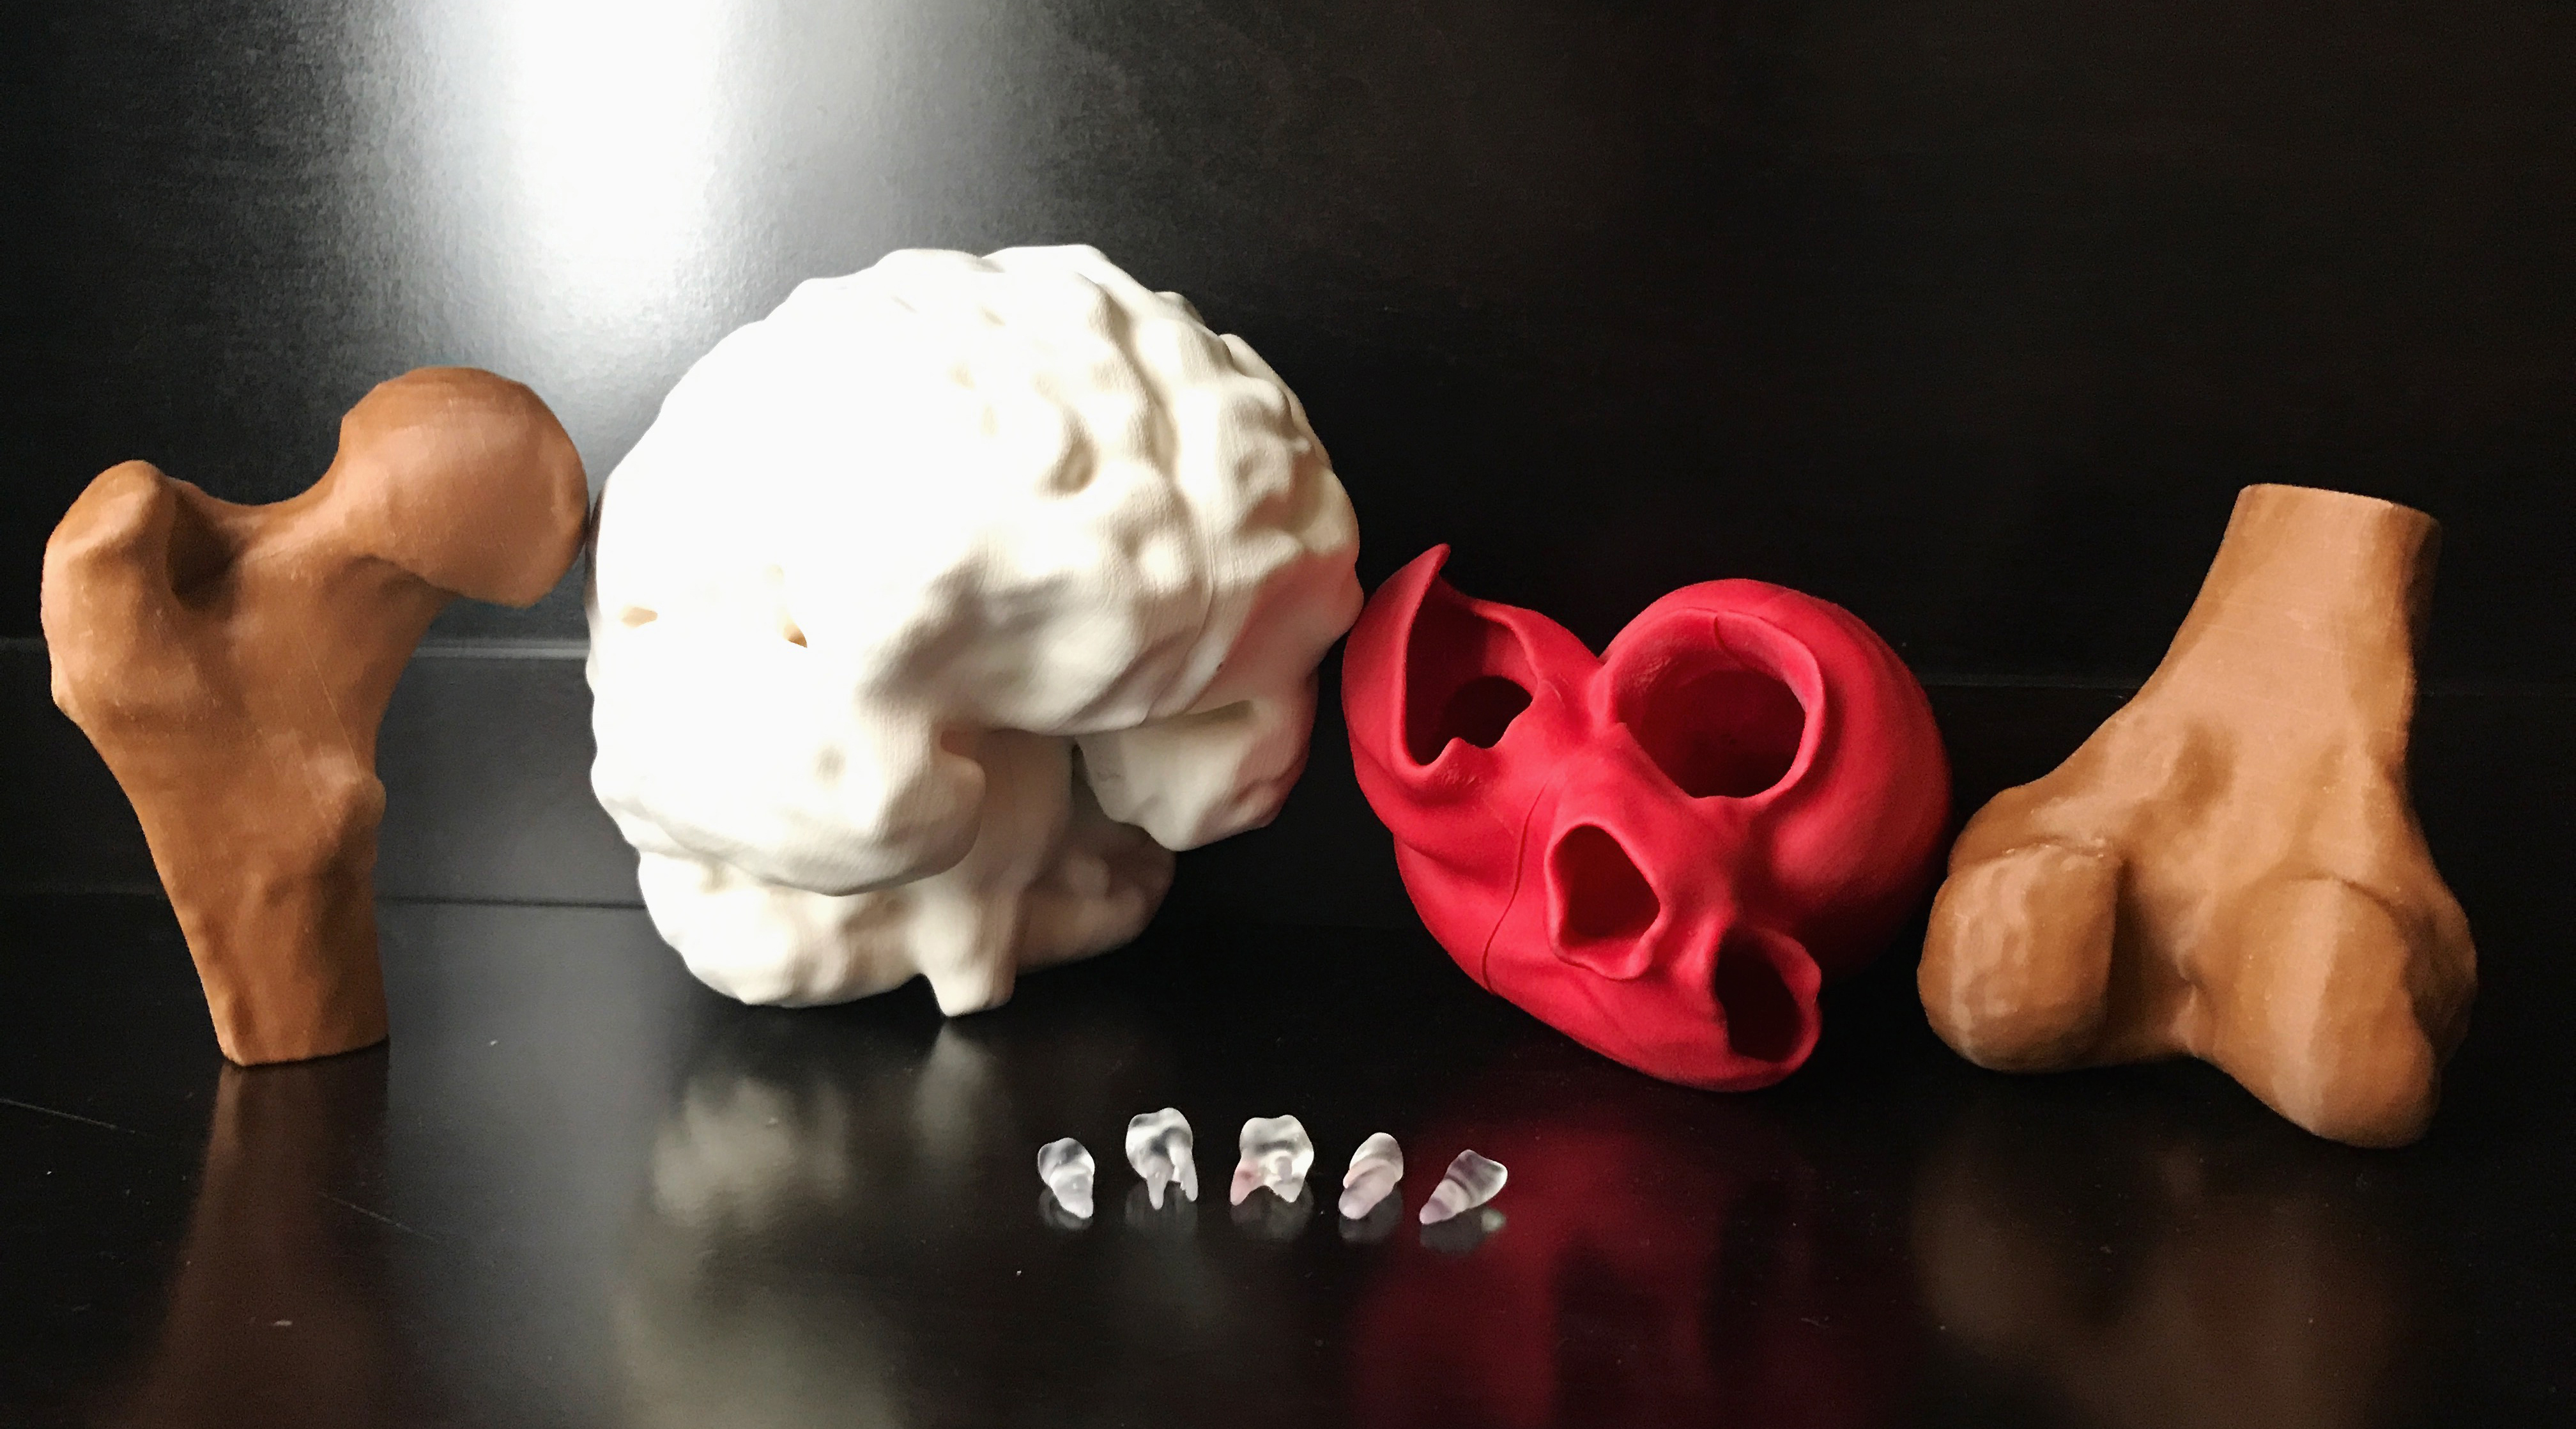
\includegraphics[width=1.0\textwidth]{media/6-3dprint/3dprint.jpg}
%
\caption{Suite of 3D-printed organs using surface meshes generated from novel image-based meshing tools}
\label{fig:3dprint}
\end{figure}

%%%%%%%%%%%%%%%%%%%%%%
%%%%%%%%%%%%%%%%%%%%%%
\section{Short Term}
\label{Short Term}

\subsection[A Polyhedral Finite Element Demonstration in Cardiac \newline Mechanics]{\texorpdfstring{A Polyhedral Finite Element Demonstration in Cardiac \newline Mechanics}{A Polyhedral Finite Element Demonstration in Cardiac \newline Mechanics}}
\label{A Polyhedral Finite Element Demonstration in Cardiac Mechanics}

like the \textit{overlay grid} hex meshing approach, suffers from having poorer quality elements near the surface than the interior. As will be discussed in next chapter, element quality for polyhedral FEM not as well defined, and may not be as egregious

direct solver is it possible if we reduce the number of DOF enough?
CLEAN THIS UP


\subsection{Improvements to Image-Based Meshing Code}
\label{Improvements to Image-Based Meshing Code}
direct surface generation from image \\
multiple materials: although plenty of work is still performed for single object meshes from images, the state of the art tools available for meshing tend to have capability for multiple materials.  \\
partial volume \\
tolerance-aware voronoi partitioning \\
use of soft segmentations/handling of partial volume effect  \\
numerical validation of segmentation and of surface --> refer to simpleware paper about geometric accuracy
inter-operator error. Assumes segmentation is perfect

\subsection{Improvements to Cardiac Mechanics Code}
\label{Improvements to Cardiac Mechanics Code}
more effort on validation of results
run PEM version in Celeris \\
BCs, etc.

%%%%%%%%%%%%%%%%%%%%%%
%%%%%%%%%%%%%%%%%%%%%%\\
\section{Long Term}
\label{Long Term}

\subsection{Simulation of Clinical Trials}
\label{Simulation of Clinical Trials}
The problem of robust patient-specific modeling has more or less been solved, even for multi-material image masks. The next step is to combine simulation related to a particular patient with statistical and/or machine learning technologies. 
A Machine Learning System to Guide Clinical Procedures in Real-Time

\subsection[Applications in Rapid Prototyping and Additive Manufacturing]{\texorpdfstring{Applications in Rapid Prototyping and Additive \newline Manufacturing}{Applications in Rapid Prototyping and Additive \newline Manufacturing}}
\label{Applications in Rapid Prototyping and Additive Manufacturing}


